% questions.tex —— 2005 年·普通高等学校招生考试·北京卷·理科 · 题目内容片段（无答案）
% 由 tools/generate_projects.py 依来源总账自 2005/2005_数学真题_北京理科_试题.md 生成，勿手改（改源 MD 后重跑）

\gkpart{一、选择题：本大题共 8 小题，每小题 5 分，共 40 分．在每小题给出的四个选项中，只有一项是符合题目要求的．}

\begin{question}
\gkti{1}设全集 $U = \mathbb{R}$，集合 $M = \{x \mid x > 1\}$，$P = \{x \mid x^2 > 1\}$，则下列关系中正确的是\mbox{（　　）}

\begin{gkopts}(2)
\task A．$M = P$
\task B．$P \subsetneqq M$
\task C．$M \subsetneqq P$
\task D．$\complement_U M \cap P = \varnothing$
\end{gkopts}

\end{question}
\begin{question}
\gkti{2}“$m = \dfrac{1}{2}$”是“直线 $(m+2)x + 3my + 1 = 0$ 与直线 $(m-2)x + (m+2)y - 3 = 0$ 相互垂直”的\mbox{（　　）}

\begin{gkopts}(2)
\task A．充分必要条件
\task B．充分而不必要条件
\task C．必要而不充分条件
\task D．既不充分也不必要条件
\end{gkopts}

\end{question}
\begin{question}
\gkti{3}若 $|\vec{a}| = 1$，$|\vec{b}| = 2$，$\vec{c} = \vec{a} + \vec{b}$，且 $\vec{c} \perp \vec{a}$，则向量 $\vec{a}$ 与 $\vec{b}$ 的夹角为\mbox{（　　）}

\begin{gkopts}(4)
\task A．$30^\circ$
\task B．$60^\circ$
\task C．$120^\circ$
\task D．$150^\circ$
\end{gkopts}

\end{question}
\begin{question}
\gkti{4}从原点向圆 $x^2 + y^2 - 12y + 27 = 0$ 作两条切线，则该圆夹在两条切线间的劣弧长为\mbox{（　　）}

\begin{gkopts}(4)
\task A．$\pi$
\task B．$2\pi$
\task C．$4\pi$
\task D．$6\pi$
\end{gkopts}

\end{question}
\begin{question}
\gkti{5}对任意的锐角 $\alpha, \beta$，下列不等关系中正确的是\mbox{（　　）}

\begin{gkopts}(1)
\task A．$\sin(\alpha + \beta) > \sin\alpha + \sin\beta$
\task B．$\sin(\alpha + \beta) > \cos\alpha + \cos\beta$
\task C．$\cos(\alpha + \beta) < \sin\alpha + \sin\beta$
\task D．$\cos(\alpha + \beta) < \cos\alpha + \cos\beta$
\end{gkopts}

\end{question}
\begin{question}
\gkti{6}在正四面体 $P - ABC$ 中，$D, E, F$ 分别是 $AB, BC, CA$ 的中点，下面四个结论中不成立的是\mbox{（　　）}

\begin{gkopts}(2)
\task A．$BC \parallel \text{\text{平面} } PDF$
\task B．$DF \perp \text{\text{平面} } PAE$
\task C．平面 $PDF \perp$ 平面 $ABC$
\task D．平面 $PAE \perp$ 平面 $ABC$
\end{gkopts}

\end{question}
\begin{question}
\gkti{7}北京《财富》全球论坛期间，某高校有 14 名志愿者参加接待工作，若每天早、中、晚三班，每班 4 人，每人每天最多值一班，则开幕式当天不同的排班种数为\mbox{（　　）}

\begin{gkopts}(1)
\task A．$\mathrm{C}_{14}^{12}\mathrm{C}_{12}^4\mathrm{C}_8^4$
\task B．$\mathrm{C}_{14}^{12}\mathrm{A}_{12}^4\mathrm{A}_8^4$
\task C．$\dfrac{\mathrm{C}_{14}^{12}\mathrm{C}_{12}^4\mathrm{C}_8^4}{\mathrm{A}_3^3}$
\task D．$\mathrm{C}_{14}^{12}\mathrm{C}_{12}^4\mathrm{C}_8^4\mathrm{A}_3^3$
\end{gkopts}

\end{question}
\begin{question}
\gkti{8}函数 $f(x) = \dfrac{\sqrt{1 - \cos 2x}}{\cos x}$\mbox{（　　）}

\begin{gkopts}(1)
\task A．在 $\left[0, \dfrac{\pi}{2}\right)$，$\left(\dfrac{\pi}{2}, \pi\right]$ 上递增，在 $\left[\pi, \dfrac{3\pi}{2}\right)$，$\left(\dfrac{3\pi}{2}, 2\pi\right]$ 上递减
\task B．在 $\left[0, \dfrac{\pi}{2}\right)$，$\left(\pi, \dfrac{3\pi}{2}\right]$ 上递增，在 $\left[\dfrac{\pi}{2}, \pi\right)$，$\left(\dfrac{3\pi}{2}, 2\pi\right]$ 上递减
\task C．在 $\left(\dfrac{\pi}{2}, \pi\right]$，$\left(\dfrac{3\pi}{2}, 2\pi\right]$ 上递增，在 $\left[0, \dfrac{\pi}{2}\right)$，$\left(\pi, \dfrac{3\pi}{2}\right]$ 上递减
\task D．在 $\left[0, \dfrac{3\pi}{2}\right)$，$\left(\dfrac{3\pi}{2}, \pi\right]$ 上递增，在 $\left[0, \dfrac{\pi}{2}\right)$，$\left(\dfrac{\pi}{2}, 2\pi\right]$ 上递减
\end{gkopts}

\end{question}
\gkpart{二、填空题：本大题共 6 小题，每小题 5 分，共 30 分．把答案填在题中横线上．}

\begin{question}
\gkti{9}若 $z_1 = a + 2\mathrm{i}$，$z_2 = 3 - 4\mathrm{i}$，且 $\dfrac{z_1}{z_2}$ 为纯虚数，则实数 $a$ 的值为 $\underline{\hspace{1.5cm}}$．

\end{question}
\begin{question}
\gkti{10}已知 $\tan\dfrac{\alpha}{2} = 2$，则 $\tan\alpha$ 的值为 $\underline{\hspace{1.5cm}}$，$\tan\left(\alpha + \dfrac{\pi}{4}\right)$ 的值为 $\underline{\hspace{1.5cm}}$．

\end{question}
\begin{question}
\gkti{11}$\left(x - \dfrac{1}{x}\right)^6$ 的展开式中的常数项是 $\underline{\hspace{1.5cm}}$．（用数字作答）

\end{question}
\begin{question}
\gkti{12}过原点作曲线 $y = \mathrm{e}^x$ 的切线，则切点的坐标为 $\underline{\hspace{1.5cm}}$，切线的斜率为 $\underline{\hspace{1.5cm}}$．

\end{question}
\begin{question}
\gkti{13}对于函数 $f(x)$ 定义域中任意的 $x_1, x_2$（$x_1 \neq x_2$），有如下结论：
① $f(x_1 + x_2) = f(x_1) \cdot f(x_2)$；
② $f(x_1 \cdot x_2) = f(x_1) + f(x_2)$；
③ $\dfrac{f(x_1) - f(x_2)}{x_1 - x_2} > 0$；
④ $f\left(\dfrac{x_1 + x_2}{2}\right) < \dfrac{f(x_1) + f(x_2)}{2}$．
当 $f(x) = \lg x$ 时，上述结论中正确结论的序号是 $\underline{\hspace{1.5cm}}$．

\end{question}
\begin{question}
\gkti{14}已知 $n$ 次多项式 $P_n(x) = a_0 x^n + a_1 x^{n-1} + \dots + a_{n-1} x + a_n$．
如果在一种算法中，计算 $x_0^k$（$k = 2, 3, 4, \dots, n$）的值需要 $k - 1$ 次乘法，计算 $P_3(x_0)$ 的值共需要 9 次运算（6 次乘法，3 次加法），那么计算 $P_{10}(x_0)$ 的值共需要 $\underline{\hspace{1.5cm}}$ 次运算．
下面给出一种减少运算次数的算法：$P_0(x) = a_0$，$P_{k+1}(x) = x P_k(x) + a_{k+1}$（$k = 0, 1, 2, \dots, n-1$）．利用该算法，计算 $P_3(x_0)$ 的值共需要 6 次运算，计算 $P_{10}(x_0)$ 的值共需要 $\underline{\hspace{1.5cm}}$ 次运算．

\end{question}
\gkpart{三、解答题：本大题共 6 小题，共 80 分．解答应写出文字说明，证明过程或演算步骤．}

\begin{question}
\gkti{15}（本小题满分 13 分）
已知函数 $f(x) = -x^3 + 3x^2 + 9x + a$．
(1) 求 $f(x)$ 的单调减区间；
(2) 若 $f(x)$ 在区间 $[-2, 2]$ 上的最大值为 20，求它在该区间上的最小值．

\Needspace{0.4\textheight}
\end{question}
\begin{question}
\gkti{16}（本小题满分 14 分）
如图，在直四棱柱 $ABCD - A_1B_1C_1D_1$ 中，$AB = AD = 2$，$DC = 2\sqrt{3}$，$AA_1 = \sqrt{3}$，$AD \perp DC$，$AC \perp BD$，垂足为 $E$．
(1) 求证：$BD \perp A_1C$；
(2) 求二面角 $A_1 - BD - C_1$ 的大小；
(3) 求异面直线 $AD$ 与 $BC_1$ 所成角的大小．
\nopagebreak[4]
\begin{center}% Source-faithful schematic draft: 2005 Beijing Science Q16, PDF p.1 (printed p.216).
% Source ID: src-f0ddb765f084ce6c1af531447a973cb8595d531721ee9b828b11a8a6e9af7809
% Source SHA-256: d30f41690977b3682009021e26659b6b575be781becee5243f5eabd1129636b9
\begin{tikzpicture}[line width=0.6pt, scale=1.0, every node/.style={inner sep=1.5pt}, baseline=(current bounding box.center)]
  % Height
  \def\h{1.9}

  % Coordinates of base ABCD matching original perspective
  \coordinate (A) at (-2.2, -0.6);
  \coordinate (D) at (-1.3, 0.0);
  \coordinate (B) at (-0.1, -1.2);
  \coordinate (C) at (2.4, -0.2);

  % Intersection E of AC and BD
  \coordinate (E) at (intersection of A--C and B--D);

  % Coordinates of top face A1B1C1D1
  \coordinate (A1) at ($(A)+(0,\h)$);
  \coordinate (D1) at ($(D)+(0,\h)$);
  \coordinate (B1) at ($(B)+(0,\h)$);
  \coordinate (C1) at ($(C)+(0,\h)$);

  % Dashed hidden base edges and diagonals
  \draw[dashed, line width=0.5pt] (A) -- (D);
  \draw[dashed, line width=0.5pt] (C) -- (D);
  \draw[dashed, line width=0.5pt] (A) -- (C);
  \draw[dashed, line width=0.5pt] (B) -- (D);
  \draw[dashed, line width=0.5pt] (D) -- (D1);

  % Dashed interior lines
  \draw[dashed, line width=0.5pt] (A1) -- (D);
  \draw[dashed, line width=0.5pt] (A1) -- (E);
  \draw[dashed, line width=0.5pt] (A1) -- (C);
  \draw[dashed, line width=0.5pt] (C1) -- (D);
  \draw[dashed, line width=0.5pt] (C1) -- (E);

  % Solid visible edges and lines
  \draw (A) -- (B) -- (C);
  \draw (A) -- (A1);
  \draw (B) -- (B1);
  \draw (C) -- (C1);
  \draw (A1) -- (B1) -- (C1) -- (D1) -- cycle;
  \draw (A1) -- (B);
  \draw (B) -- (C1);

  % Labels
  \node[below left] at (A) {$A$};
  \node[below] at (B) {$B$};
  \node[right] at (C) {$C$};
  \node[left] at (D) {$D$};
  \node[above=2pt] at (E) {$E$};
  \node[left] at (A1) {$A_1$};
  \node[above] at (B1) {$B_1$};
  \node[above right] at (C1) {$C_1$};
  \node[above left] at (D1) {$D_1$};
\end{tikzpicture}
\end{center}
\nopagebreak[4]
\end{question}
\begin{question}
\gkti{17}（本小题满分 13 分）
甲、乙两人各进行 3 次射击，甲每次击中目标的概率为 $\dfrac{1}{2}$，乙每次击中目标的概率为 $\dfrac{2}{3}$．
(1) 记甲击中目标的次数为 $\xi$，求 $\xi$ 的概率分布及数学期望 $E\xi$；
(2) 求乙至多击中目标 2 次的概率；
(3) 求甲恰好比乙多击中目标 2 次的概率．

\Needspace{0.4\textheight}
\end{question}
\begin{question}
\gkti{18}（本小题满分 13 分）
如图，直线 $l_1 : y = kx$（$k > 0$）与直线 $l_2 : y = -kx$ 之间的阴影区域（不含边界）记为 $W$，其左半部分记为 $W_1$，右半部分记为 $W_2$．
(1) 分别用不等式组表示 $W_1$ 和 $W_2$；
(2) 若区域 $W$ 中的动点 $P(x, y)$ 到 $l_1, l_2$ 的距离之积等于 $d^2$，求点 $P$ 的轨迹 $C$ 的方程；
(3) 设不过原点 $O$ 的直线 $l$ 与 (2) 中的曲线 $C$ 相交于 $M_1, M_2$ 两点，且与 $l_1, l_2$ 分别交于 $M_3, M_4$ 两点．求证：$\triangle OM_1M_2$ 的重心与 $\triangle OM_3M_4$ 的重心重合．
\nopagebreak[4]
\begin{center}% Source-faithful schematic draft: 2005 Beijing Science Q18, PDF p.2 (printed p.217).
% Source ID: src-f0ddb765f084ce6c1af531447a973cb8595d531721ee9b828b11a8a6e9af7809
% Source SHA-256: d30f41690977b3682009021e26659b6b575be781becee5243f5eabd1129636b9
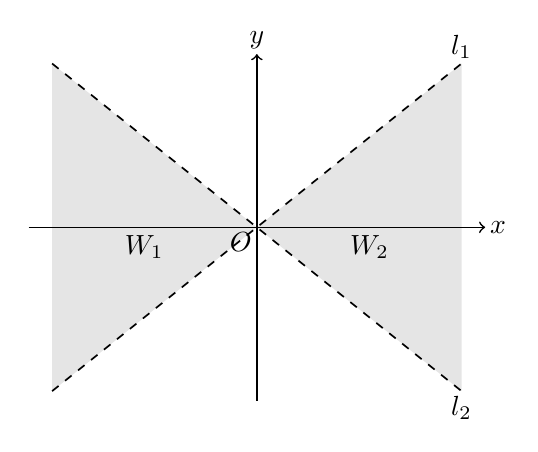
\begin{tikzpicture}[line width=0.6pt, scale=1.0, every node/.style={inner sep=1.5pt}, baseline=(current bounding box.center)]
  % Axes limits
  \def\xmax{2.6}
  \def\ymax{2.0}
  \def\k{0.8}

  % Shaded regions W1 and W2
  \fill[gray!20] (-\xmax, {-\k*\xmax}) -- (0, 0) -- (-\xmax, {\k*\xmax}) -- cycle;
  \fill[gray!20] (\xmax, {-\k*\xmax}) -- (0, 0) -- (\xmax, {\k*\xmax}) -- cycle;

  % Boundary dashed lines l1 and l2
  \draw[dashed, line width=0.6pt] (-\xmax, {-\k*\xmax}) -- (\xmax, {\k*\xmax}) node[above] {$l_1$};
  \draw[dashed, line width=0.6pt] (-\xmax, {\k*\xmax}) -- (\xmax, {-\k*\xmax}) node[below] {$l_2$};

  % Solid coordinate axes
  \draw[->] (-\xmax-0.3, 0) -- (\xmax+0.3, 0) node[right] {$x$};
  \draw[->] (0, -\ymax-0.2) -- (0, \ymax+0.2) node[above] {$y$};

  % Labels
  \node[below left] at (0, 0) {$O$};
  \node at ({-0.55*\xmax}, -0.25) {$W_1$};
  \node at ({0.55*\xmax}, -0.25) {$W_2$};
\end{tikzpicture}
\end{center}
\nopagebreak[4]
\end{question}
\begin{question}
\gkti{19}（本小题满分 14 分）
\Needspace{5\baselineskip}
设数列 $\{a_n\}$ 的首项 $a_1 = a \neq \dfrac{1}{4}$，且
\nopagebreak[4]
\[
a_{n+1} = \begin{cases} \dfrac{1}{2}a_n, & n \text{ \text{为偶数}}, \\[6pt] a_n + \dfrac{1}{4}, & n \text{ \text{为奇数}}. \end{cases}
\]
记 $b_n = a_{2n-1} - \dfrac{1}{4}$，$n = 1, 2, 3, \dots$．
(1) 求 $a_2, a_3$；
(2) 判断数列 $\{b_n\}$ 是否为等比数列，并证明你的结论；
(3) 求 $\lim\limits_{n \to \infty} (b_1 + b_2 + \dots + b_n)$．

\end{question}
\begin{question}
\gkti{20}（本小题满分 13 分）
设 $f(x)$ 是定义在 $[0, 1]$ 上的函数，若存在 $x^* \in (0, 1)$，使得 $f(x)$ 在 $[0, x^*]$ 上单调递增，在 $[x^*, 1]$ 上单调递减，则称 $f(x)$ 为 $[0, 1]$ 上的单峰函数，$x^*$ 为峰点，包含峰点的区间为含峰区间．对任意的 $[0, 1]$ 上的单峰函数 $f(x)$，下面研究缩短其含峰区间长度的方法．
(1) 证明：对任意的 $x_1, x_2 \in (0, 1)$，$x_1 < x_2$，若 $f(x_1) \geqslant f(x_2)$，则 $(0, x_2)$ 为含峰区间；若 $f(x_1) \leqslant f(x_2)$，则 $(x_1, 1)$ 为含峰区间；
(2) 对给定的 $r$（$0 < r < 0.5$），证明：存在 $x_1, x_2 \in (0, 1)$，满足 $x_2 - x_1 \geqslant 2r$，使得由 (1) 所确定的含峰区间的长度不大于 $0.5 + r$；
(3) 选取 $x_1, x_2 \in (0, 1)$，$x_1 < x_2$，由 (1) 可确定含峰区间为 $(0, x_2)$ 或 $(x_1, 1)$，在所得的含峰区间内选取 $x_3$，由 $x_3$ 与 $x_1$ 或 $x_3$ 与 $x_2$ 类似地可确定一个新的含峰区间，在第一次确定的含峰区间为 $(0, x_2)$ 的情况下，试确定 $x_1, x_2, x_3$ 的值，满足两两之差的绝对值不小于 $0.02$，且使得新的含峰区间的长度缩短到 $0.34$．
注：区间长度等于区间的右端点与左端点之差．

\end{question}